\documentclass[14pt]{extarticle}
% Full article preamble (duplicated, no common file)
\usepackage{fontspec}
\usepackage[a4paper,margin=2.5cm,includefoot]{geometry}
\usepackage{polyglossia}
\usepackage{amsmath}
\usepackage{amssymb}
\usepackage{xcolor}
\usepackage{fancyhdr}
\usepackage{graphicx}
\usepackage{listings}
\usepackage[most]{tcolorbox}
\usepackage{pifont}
\usepackage{enumitem}
\usepackage{titlesec}
\usepackage[bottom]{footmisc}
\usepackage{titling}
\usepackage{minted}
\usepackage{etoolbox}
\usepackage{array}
\usepackage{extsizes}

\newfontfamily\emoji{Segoe UI Emoji}

\pagestyle{fancy}

\setmainlanguage[numerals=western]{arabic}
\setotherlanguage{english}
\newfontfamily\arabicfont[Script=Arabic]{Amiri}
\newfontfamily\arabicfonttt[Script=Arabic]{Courier New}

\lstset{
  language=[Sharp]C,
  numbers=left,
  stepnumber=1,
  numbersep=8pt,
  frame=single,
  basicstyle=\ttfamily\small,
  keywordstyle=\color{blue},
  stringstyle=\color{red},
  commentstyle=\color{green!50!black}
}

\newif\ifdetailed
\ifdefined\setdetailed
  \setdetailed
\fi

\newif\ifwithsols
\ifdefined\setwithsols
  \setwithsols
\fi

% unified tcolorboxes for articles
\tcbset{colback=white, colframe=black, fonttitle=\bfseries, boxrule=0.8pt}
\newtcolorbox{boxDef}[1][]{colback=blue!5!white,colframe=blue!75!black,
  title={{\emoji📘} تعريف\ifx\\#1\\\else ~#1\fi :}}
\newtcolorbox{boxExercise}[1][]{colback=cyan!5!white,colframe=cyan!70!black,
  title={{\emoji🧩} تمرين\ifx\\#1\\\else ~#1\fi :}}
\newtcolorbox{boxExample}[1][]{colback=yellow!5!white,colframe=orange!90!black,
  title={{\emoji📝} مثال\ifx\\#1\\\else ~#1\fi :}}
\newtcolorbox{boxNote}[1][]{colback=gray!10!white,colframe=black,
  title={{\emoji✨} ملاحظة\ifx\\#1\\\else ~#1\fi :}}
\newtcolorbox{boxAttention}[1][]{colback=magenta!10!white,colframe=magenta!80!black,
  title={{\emoji🔔} تنبيه\ifx\\#1\\\else ~#1\fi :}}
\newtcolorbox{boxWarning}[1][]{colback=red!5!white,colframe=red!75!black,
  title={{\emoji⚡} ملاحظة هامة\ifx\\#1\\\else ~#1\fi :}}
\newtcolorbox{boxSolution}[1][]{colback=green!5!white,colframe=green!60!black,
  title={{\emoji✅} حل\ifx\\#1\\\else ~#1\fi :}}
\newtcolorbox{boxSymbol}[1][]{colback=purple!5!white,colframe=purple!70!black,
  title={{\emoji🔣} رمز\ifx\\#1\\\else ~#1\fi :}}

\tcbset{simplecode/.style={ colback=gray!5, colframe=black!50, boxrule=0.4pt, arc=2pt, left=4pt,right=4pt,top=4pt,bottom=4pt}}
\newenvironment{boxCode}{\begin{tcolorbox}[simplecode]}{\end{tcolorbox}}

\newcolumntype{C}[1]{>{\centering\arraybackslash}p{#1}}

% redefine spaces after titles
\makeatletter
\renewcommand{\@maketitle}{%
  \begin{center}
    {\huge \bfseries \@title \par}%
    \vskip 0.2em % space between title and author
    {\large \@author \par}%
    % \vskip 0.2em % space between author and date
    % {\normalsize \@date \par}%
  \end{center}
}
\makeatother

\fancyhf{} % clear default
\fancypagestyle{plain}{
  \fancyhf{}
  \fancyhead[L]{مدرسة التسامح الشاملة}
  % \fancyhead[L]{
\includegraphics[height=1cm]{../../../images/logoTasamoh.png}}
  \fancyhead[R]{الأستاذ محمود اغبارية}
  \fancyfoot[C]{\thepage}
}

\fancyhead[L]{مدرسة التسامح الشاملة}
\fancyhead[R]{الأستاذ محمود اغبارية}
\fancyfoot[C]{\thepage}
% \date{\today}

\setcounter{tocdepth}{3} % only section subsection and subsubsection in TOC


% ----------------------


% \begin{document}

% \maketitle

% % \clearpage  % start TOC on a new page
% % \renewcommand{\contentsname}{جدول المحتويات}
% % \tableofcontents
% % \clearpage

% \part*{part 1} % the * prevents numbering
% \section*{مقدمة}
% \subsection*{مثال رياضي}
% \subsubsection*{مثال فرعي}
% \paragraph*{ paragraph 1}
% \subparagraph*{sub paragraph 1}

% \ifdetailed
% \begin{english}
% \begin{minted}{csharp}
% // C# Example
% \end{minted}
% \end{english}
% \fi

% OLD WAY
% \ifdetailed
% \begin{english}
% \begin{lstlisting}
% // C# Example
% \end{lstlisting}
% \end{english}
% \fi

% % 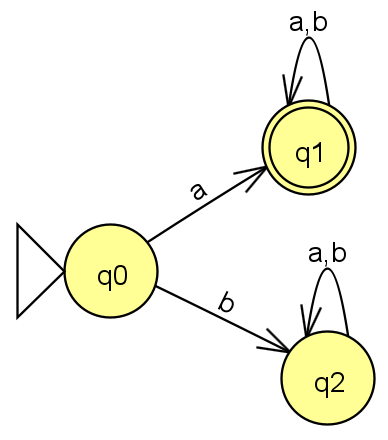
\includegraphics[width=0.2\textwidth]{../../../images/DFAs/ex1_q1.png}



% \vspace{3cm}
% \begin{flushleft}
% أرجو لكم وقتًا ممتعًا.

% الأستاذ محمود اغبارية.
% \end{flushleft}


% \end{document}


\title{اختبار شهري للصف 10-10}

\begin{document}
\maketitle
% \thispagestyle{fancy}

\ifwithsols
\else
\begin{boxCode}
    \begin{itemize}[nosep]
        \item \textbf{أجب عن جميع الأسئلة}
        \item الوقت المخصص: ساعة ونصف.
        \item يسمح باستخدام كل مادة مساعة، عدا الآلة التي يمكن برمجتها.
        \item أجب بلغة \textenglish{C\#} فقط.
        \item اكتب بقلم حبر فقط، وبخط واضح.
        \item الحل على ورقة خارجية، لا تنسَ كتابة اسمك
    \end{itemize}
\end{boxCode}
\fi

\vspace{1cm}

\begin{enumerate}[itemsep=3em]

\item
اكتب مقطع برنامج يستقبل عددين صحيحين ويطبع \textenglish{"Consecutive"} إذا كانا متتاليين، و \textenglish{"Not Consecutive"} إذا لم يكونا متتاليين.

\ifwithsols
\begin{boxSolution}[1]
\begin{english}
\begin{minted}{csharp}
int a = int.Parse(Console.ReadLine());
int b = int.Parse(Console.ReadLine());
if (Math.Abs(a - b) == 1)
{
    Console.WriteLine("Consecutive");
}
else
{
    Console.WriteLine("Not Consecutive");
}
\end{minted}
\end{english}
\end{boxSolution}
\begin{boxSolution}[2]
\begin{english}
\begin{minted}{csharp}
int a = int.Parse(Console.ReadLine());
int b = int.Parse(Console.ReadLine());
if ((Math.Max(a, b) - Math.Min(a, b)) == 1)
{
    Console.WriteLine("Consecutive");
}
else
{
    Console.WriteLine("Not Consecutive");
}
\end{minted}
\end{english}
\end{boxSolution}
\clearpage
\fi

\item
اكتب مقطع برنامج يستقبل عددًا صحيحا موجبًا، ويطبع الرّقم الزوجي التالي لهذا الرقم.\\
\textbf{مثال}: إذا استقبل العدد 5، يطبع البرنامج 6. وإذا استقبل 6 يطبع البرنامج 8.

\ifwithsols
\begin{boxSolution}[1]
\begin{english}
\begin{minted}{csharp}
int x = int.Parse(Console.ReadLine());
int nextEven;
if (x % 2 == 0)
{
    nextEven = x + 2;
}
else
{
    nextEven = x + 1;
}
Console.WriteLine(nextEven);
\end{minted}
\end{english}
\end{boxSolution}
\begin{boxSolution}[2]
\begin{english}
\begin{minted}{csharp}
int x = int.Parse(Console.ReadLine());
int nextEven = x + 2 - (x % 2);
Console.WriteLine(nextEven);
\end{minted}
\end{english}
\end{boxSolution}
\clearpage
\fi

\item
اكتب مقطع برنامج يستقبل عددين صحيحين وموجبين، العدد الأول مؤلف من منزلتين والعدد الثاني مؤلف من منزلة واحدة. \\
على البرنامج أن يطبع \textenglish{Yes} إذا كان العدد الثاني هو إحدى منازل العدد الأول. ويطبع \textenglish{No} في باقي الحالات. \\
لا حاجة لفحص الأعداد المعطاة - افترض أنّها صحيحة والأول من منزلتين والثاني من منزلة واحدة.

\textbf{مثال}: إذا كان العدد الأول 35، والعدد الثاني 3 فعلى البرنامج أن يطبع \textenglish{Yes}. \\
إذا كان العدد الأول 35، والعدد الثاني 7 فعلى البرنامج أن يطبع \textenglish{No}. \\


\ifwithsols
\begin{boxSolution}
\begin{english}
\begin{minted}{csharp}
int n = int.Parse(Console.ReadLine());
int d = int.Parse(Console.ReadLine());
int tens = n / 10;
int ones = n % 10;
if (d == tens || d == ones)
{
    Console.WriteLine("Yes");
}
else
{
    Console.WriteLine("No");
}
\end{minted}
\end{english}
\end{boxSolution}
\fi

\clearpage
\item
تتبع مقطع الكود التالي ثم املأ الجدول الذي بعده:

\begin{boxCode}
\begin{english}
\begin{minted}{csharp}
int n = int.Parse(Console.ReadLine());
int a = n / 100;
int b = n % 10;
int result = a * 10 + b;
Console.WriteLine(result);
\end{minted}
\end{english}
\end{boxCode}



\begin{enumerate}
    \item
    \textbf{املأ الجدول التالي:} لكل واحدة من قيم $n$، اكتب ماذا تكون قيمة $a, b$ وما هي القيمة التي يطبعها البرنامج:
\begin{center}

\begin{tabular}{|C{2cm}|C{3cm}|C{3cm}|C{3cm}|C{3cm}|}
\hline
\large{\textbf{$n$}} & \large{\textbf{$a$}} & \large{\textbf{$b$}} & \large{\textenglish{\textbf{result}}} \\
\hline
7654 &  &  &  \\
\hline
32154 &  &  &  \\
\hline
8111 &  &  &  \\
\hline
54 &  &  &  \\
\hline
1 &  &  &  \\
\hline
\end{tabular}
\end{center}

\item
ما هي وظيفة البرنامج أعلاه؟ (أجب بسطر واحد)

\item
أعط قيمة لـ $n$ تجعل البرنامج يطبع $321$.
\end{enumerate}

\ifwithsols
\begin{boxSolution}
\begin{enumerate}
\item القيم المطلوبة في الجدول:
\begin{center}
\begin{tabular}{|C{2cm}|C{3cm}|C{3cm}|C{3cm}|}
\hline
\large{\textbf{$n$}} & \large{\textbf{$a$}} & \large{\textbf{$b$}} & \large{\textenglish{\textbf{result}}} \\
\hline
7654 & 76 & 4 & 764 \\
\hline
32154 & 321 & 4 & 3214 \\
\hline
8111 & 81 & 1 & 811 \\
\hline
54 & 0 & 4 & 4 \\
\hline
1 & 0 & 1 & 1 \\
\hline
\end{tabular}
\end{center}

\item وظيفة البرنامج: حذف منزلة العشرات من العدد $n$ (أي حذف الرقم الثاني من اليمين).

\item مثال لقيمة تجعل الناتج $321$: على سبيل المثال $n=3211$.
\end{enumerate}
\end{boxSolution}
\fi

\clearpage


\item
معطاة الدالة التالية:
\[ f(x) = \frac{x^5 - 3}{\sqrt{25 - x^2}} \]

اكتب مقطع برنامج يستقبل من المستخدم عددًا عشريًّا يمثّل قيمة $x$ ويطبع قيمة $f(x)$. \\
لكن علينا الانتباه لمجال تعريف الدالة، لذلك:
\begin{itemize}
    \item إذا كان $x = 5$ على البرنامج أن يطبع "خطأ: قسمة  على صفر"، \\ \textenglish{("ERROR: division by 0")}.
    \item إذا كان $x$ أكبر من $5$ أو أصغر من $-5$ على البرنامج أن يطبع: "خطأ: جذر عدد سالب"، \textenglish{("ERROR: Negative square root")}.
    \item في باقي الحالات (أي إذا كان $x$ بين $5$ و $-5$) ، على البرنامج أن يطبع قيمة $f(x)$.
\end{itemize}

\ifwithsols
\begin{boxSolution}
\begin{english}
\begin{minted}{csharp}
int x = int.Parse(Console.ReadLine());
if (x == 5)
    {
        Console.WriteLine("ERROR: division by 0");
    }
else if (x > 5 || x < -5)
    {
        Console.WriteLine("ERROR: Negative square root");
    }
else
    {
        double x5 = Math.Pow(x,5);
        double s = Math.Sqrt(25 - Math.Pow(x,2));
        double fx = (x5 - 3) / s;
        Console.WriteLine(fx);
    }
\end{minted}
\end{english}
\end{boxSolution}
\fi

\clearpage
\item
كل مثلث في المستوى يجب أن يحقق قانون بناء المثلث وهو أنّ مجموع \textbf{كل} ضلعين أكبر من الثالث. \\
 أي إذا كانت أضلاعه $a, b, c$ فإنّه يجب أن يحقق كل الشروط التالية:
\[ a + b > c ,  \qquad a + c > b ,  \qquad b + c > a \]

\textbf{اكتب مقطع برنامج} يفحص إذا كانت هذه الأطوال تحقق قانون بناء المثلث أم لا (لا حاجة لاستقبال الأطوال من المستخدم). \\
إذا كانت تحقق قانون بناء المثلث فعلى البرنامج أن يطبع \textenglish{"Legal"}. \\
وإلا فإنّه يطبع \textenglish{"Not Legal"}.

\textbf{مثال}: الأطوال $3, 4, 5$ تحقق قانون بناء المثلث، لأنّ $3 + 4 > 5$ و $3 + 5 > 4$ و $4 + 5 > 3$. ففي هذه الحالة على البرنامج أن يطبع \textenglish{"Legal"}. \\
أمّا الأطوال $3, 4, 9$ لا تحقق قانون بناء المثلث، لأنّ $3 + 4 < 9$، ففي هذه الحالة على البرنامج أن يطبع \textenglish{"Not Legal"}.

\ifwithsols
\begin{boxSolution}
\begin{english}
\begin{minted}{csharp}
int a = int.Parse(Console.ReadLine());
int b = int.Parse(Console.ReadLine());
int c = int.Parse(Console.ReadLine());
if ((a + b > c) && (a + c > b) && (b + c > a))
{
    Console.WriteLine("Legal");
}
else
{
    Console.WriteLine("Not Legal");
}
\end{minted}
\end{english}
\end{boxSolution}
\fi


\end{enumerate}

\vspace{3cm}
\begin{flushleft}
أرجو لكم التفوّق.

الأستاذ محمود اغبارية.
\end{flushleft}



\ifwithsols
\else
% ----------------------------------------------
% Submission page for students (to hand in)
\clearpage
\begin{center}
{\Large ورقة تسليم للطالب}
\end{center}


\noindent\textbf{الاسم:}\hspace{0.5cm}\rule{6cm}{0.6pt}

\vspace{0.5cm}

\noindent\textbf{السؤال 4 — الجدول}

\begin{center}
\begin{tabular}{|C{2cm}|C{3cm}|C{3cm}|C{3cm}|}
\hline
\Large{\textbf{$n$}} & \Large{\textbf{$a$}} & \Large{\textbf{$b$}} & \Large{\textenglish{\textbf{result}}} \\[0.5cm]
\hline
7654 &  &  &  \\[0.5cm]
\hline
32154 &  &  &  \\[0.5cm]
\hline
8111 &  &  &  \\[0.5cm]
\hline
54 &  &  &  \\[0.5cm]
\hline
1 &  &  &  \\[0.5cm]
\hline
\end{tabular}
\end{center}

\vspace{1cm}

\noindent\textbf{(ب) ما هي وظيفة البرنامج؟ (أجب بسطر واحد)}\\[1.2cm]
\rule{0.95\linewidth}{0.6pt}

\vspace{1.8cm}

\noindent\textbf{(ج) أعط قيمة لـ $n$ تجعل البرنامج يطبع $321$:}\hspace{0.5cm}\rule{6cm}{0.6pt}

\clearpage

\noindent\textbf{السؤال 5 — مخطط الحل}

\begin{boxCode}
\begin{english}
\begin{minted}{csharp}
double x = double.Parse(Console.ReadLine());

if (____________________________________)
{
    Console.WriteLine("ERROR: division by 0");
}
else if (_________________________________________)
{
    Console.WriteLine("ERROR: Negative square root");
}
else
{
    _________________________________________________;

    _________________________________________________;

    _________________________________________________;

    _________________________________________________;

    Console.WriteLine("f(x) = " + fx);
}
\end{minted}
\end{english}
\end{boxCode}

\fi

\end{document}
